
%----------------------------------------------------------------------------------------
%   Хавсралтууд эндээс эхэлнэ
%----------------------------------------------------------------------------------------
\appendix
\addcontentsline{toc}{part}{ХАВСРАЛТ}

% Хавсралтын нэр. Хавсралт гэдэг үг агуулахгүй
\chapter{Үечилсэн төлөвлөгөө}
\begin{figure}[h]
	\centering
	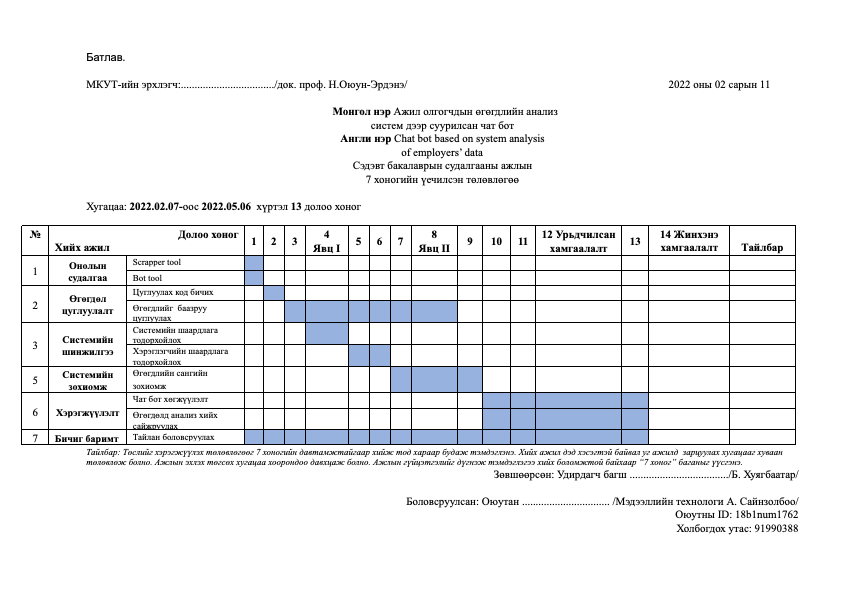
\includegraphics[width=16.5cm, angle=90]{images/plan.png}
	\caption{Бакалаврын судалгааны ажлын үечилсэн төлөвлөгөө}
	\label{fig:plan01}
\end{figure}
% Хавсралтын нэр. Хавсралт гэдэг үг агуулахгүй
\chapter{Кодын хэрэгжүүлэлт}

\section{Өгөгдөл цугуулалт}
Өгөгдөл цуглуулах програм нь дараах бүтэцтэй байх бөгөөд assets доторх кодууд нь үндсэн кодыг ажлуулахад туслах функцууд байна.
\begin{figure}[h]
	\centering
	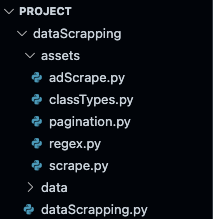
\includegraphics[width=5cm]{images/folderStructure.png}
	\caption{Фолдерийн бүтэц}
	\label{fig:plan01}
\end{figure}
\subsection{Үндсэн өгөгдлийг цуглуулах эх код}
\lstinputlisting[language=Python, caption=Бүх өгөгдлийг цуглуулах - dataScrapping.py]{code/dataScrapping.py}
\subsection{Нэг зарын шаардлагатай бүх мэдээллийг цуглуулах код}
\lstinputlisting[language=Python, caption=Нэг зарын өгөгдлийг цуглуулах - adScrape.py]{code/adScrape.py}
\subsection{Цуглуулах өгөгдлийн төрөл}
\lstinputlisting[language=Python, caption=Өгөгдлийн төрөл - classTypes.py]{code/classTypes.py}
\subsection{BeautifulSoup scraper}
\lstinputlisting[language=Python, caption=Scrape хийх функц - scrape.py]{code/scrape.py}